% --- Section 1: Présentation ---
\section{Contexte et objectifs}
\begin{frame}{Contexte et Objectifs}
    \begin{center}
        Pipeline agentique multi expert pour la découverte de peptides \textit{in silico}
        \\
        \footnotesize{in silico: réalisé par ordinateur, sans expérimentation physique.}
        \\
        \centering
        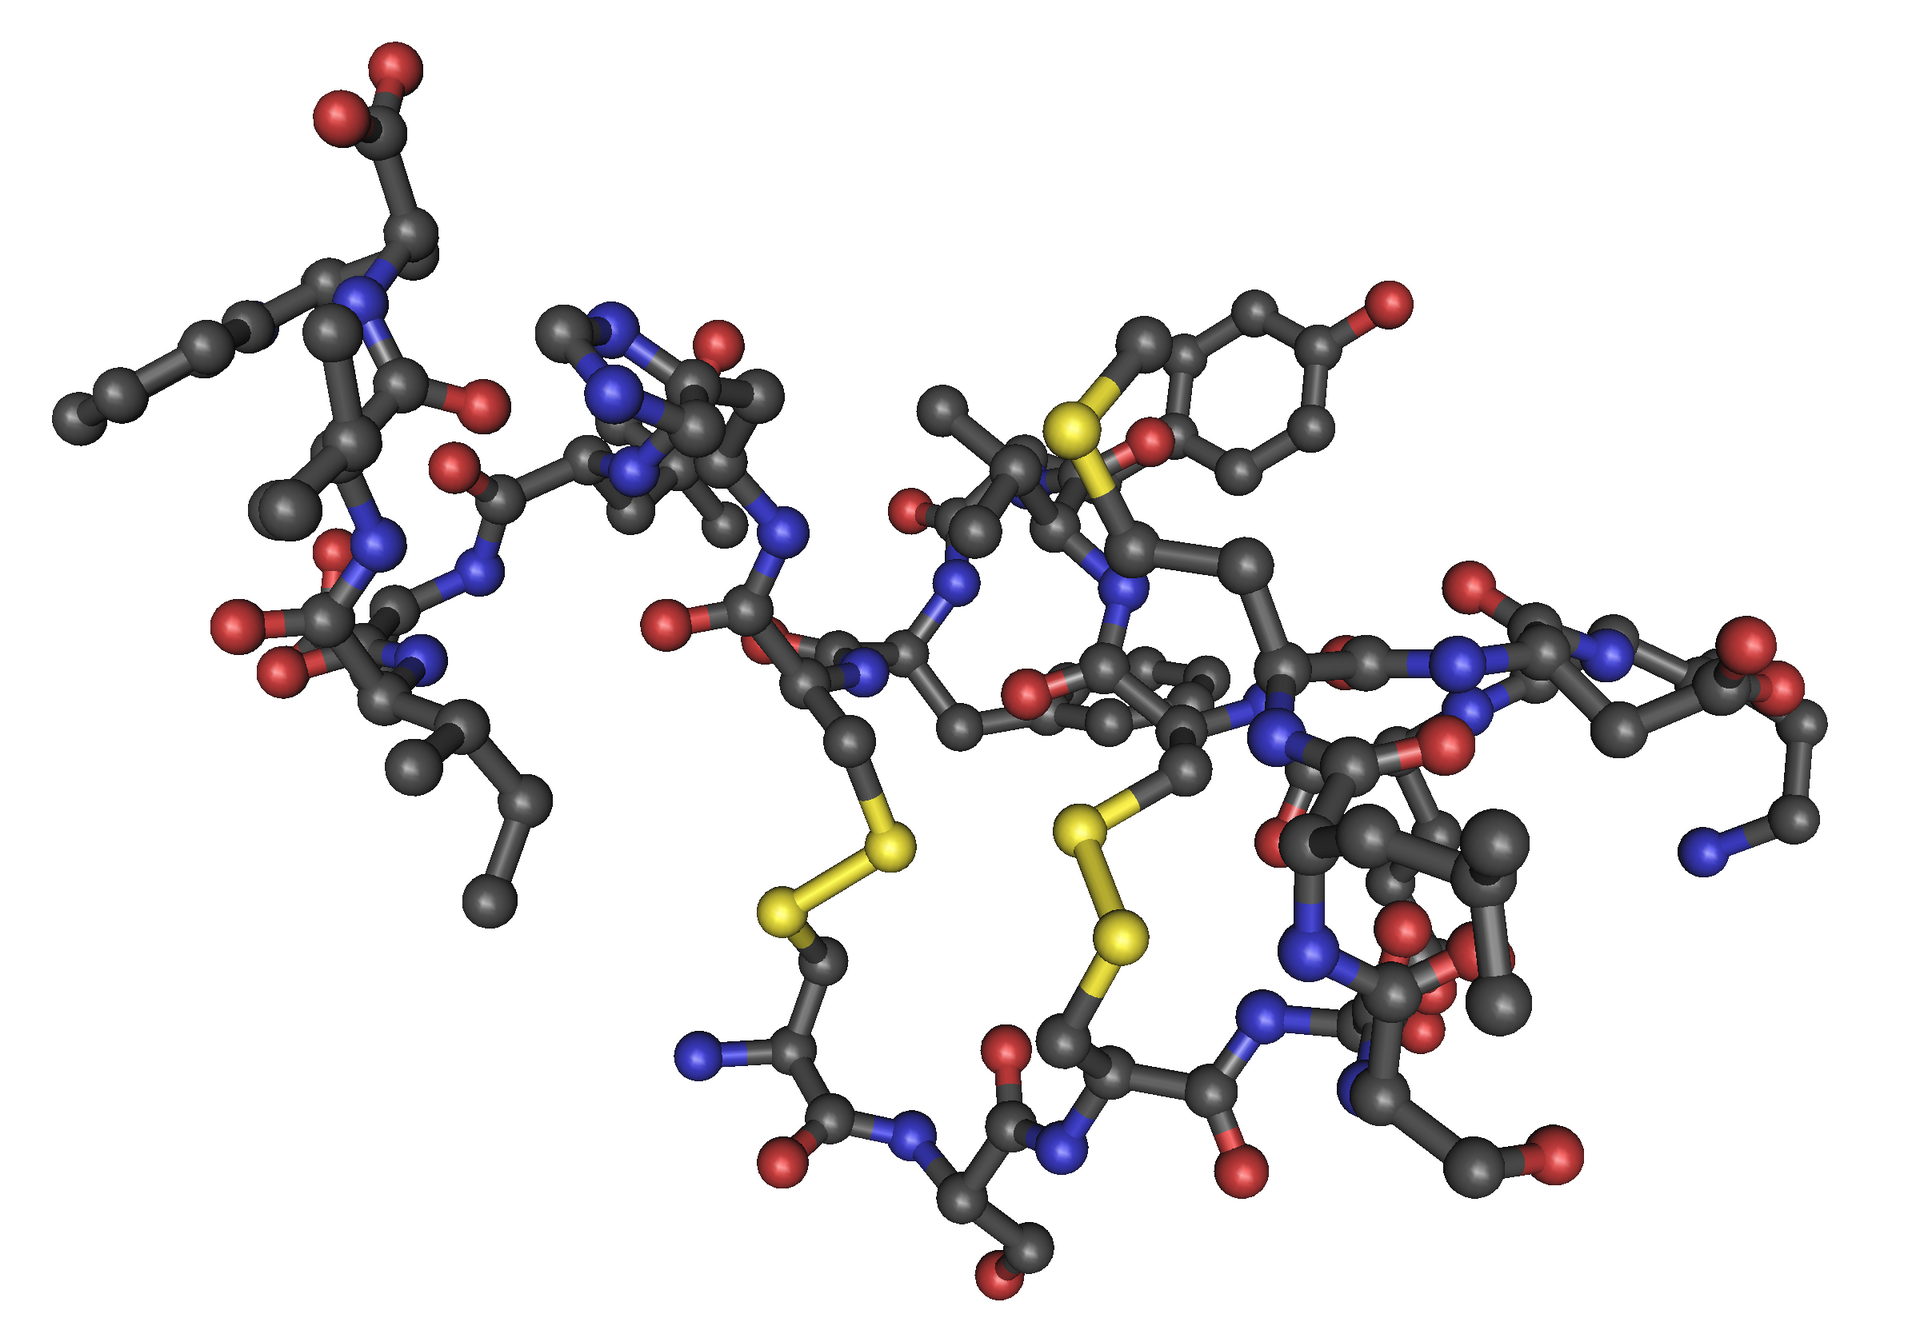
\includegraphics[height=4cm]{peptide.png}
    \end{center}
\end{frame}

\begin{frame}
    \frametitle{Peptide}
    \begin{itemize}
        \item Chaîne composée d'au plus 50 acides aminés
        \item 20 acides aminés différents
        \item Applications: médecine, agriculture, industrie
        \item Exemples: insuline, antibiotiques, hormones
    \end{itemize}

    \begin{block}{Processus de découverte actuel}
        \begin{itemize}
            \item Découverte de peptides: criblage de bibliothèques, évolution dirigée
            \item Évaluation: tests biologiques, simulations moléculaires
            \item Itération sur les resultats pour améliorer l'efficacité de la peptides
            \item Coût élevé, temps long, taux de succès faible
        \end{itemize}
    \end{block}
\end{frame}

\section{Experts et Architecture}
\begin{frame}
    \frametitle{Pipeline}
        \begin{center}
            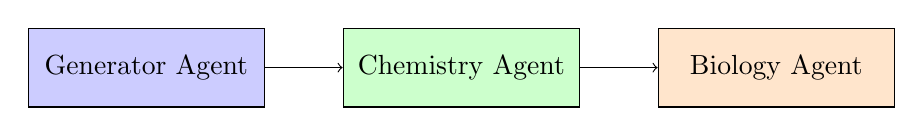
\begin{tikzpicture}
            \node[rectangle, draw, fill=blue!20, minimum width=3cm, minimum height=1cm, align=center] (gen) at (0, 0) {Generator Agent};
            \node[rectangle, draw, fill=green!20, minimum width=3cm, minimum height=1cm, align=center] (chem) at (4, 0) {Chemistry Agent};
            \node[rectangle, draw, fill=orange!20, minimum width=3cm, minimum height=1cm, align=center] (bio) at (8, 0) {Biology Agent};

            \draw[->] (gen) -- (chem);
            \draw[->] (chem) -- (bio); 
            \end{tikzpicture}
        \end{center}
\end{frame}